\documentclass[12pt,a4paper]{article}
\usepackage{ucebnice}

\title{Základní matematické poznatky}
\author{Ondřej Škubala}
\date{\today}

\begin{document}

\maketitle
\newpage

\section{Mocniny a odmocniny}

\begin{quotebox}
{„Každý problém, který jsem kdy vyřešil, se stal pravidlem, které mi pomohlo vyřešit další problémy.“}
{René Descartes}
\end{quotebox}

\begin{historicalbox}
\textbf{Historie mocnin a odmocnin}  

\smallskip
\textbf{Starověký Orient a Egypt.}  
První záznamy o počítání se čtverci a odmocninami nacházíme už ve starověké Mezopotámii. Babylonské hliněné tabulky (okolo roku 2000 př. n. l.) obsahují seznamy čísel seřazených podle jejich čtverců a druhých odmocnin. Tyto tabulky sloužily stavitelům chrámů a zeměměřičům při praktických výpočtech. V Egyptě se používaly metody „zdvojnásobování a půlení“ a odmocňování se řešilo přibližnými výpočty pomocí tabulek.

\smallskip
\textbf{Antické Řecko.}  
Řečtí matematici spojovali mocniny především s geometrií:
\begin{itemize}
    \item \emph{druhá mocnina} (\(a^2\)) byla plocha čtverce nad stranou délky \(a\),
    \item \emph{třetí mocnina} (\(a^3\)) objem krychle se stranou \(a\).
\end{itemize}
Výrazy jako \(a^4\) nebo \(a^5\) se tehdy nepoužívaly, protože neměly přímý geometrický význam.  
Pythagorejci zkoumali čtverce čísel a jejich vztah k hudbě, 
Eukleidés v „Základech“ dokázal pravidla pro odmocniny geometrickými konstrukcemi.

\smallskip
\textbf{Indie a Čína.}  
Indičtí matematici (Brahmagupta, 7. století) už pracovali s pravidly pro mocniny a 
odmocniny velmi blízkými dnešním. V Číně se v „Matematice v devíti knihách“ (1.–2. stol. n. l.) 
objevuje algoritmus pro výpočet druhé a třetí odmocniny pomocí postupného 
odhadu – obdoba dnešní metody „dělení písemně“.

\smallskip
\textbf{Arabská matematika.}  
Arabští učenci převzali řecké, indické a čínské poznatky a sjednotili je. 
Z tohoto období pochází i dnešní symbol odmocniny \(\sqrt{\ }\). 
Poprvé jej použil al-Hasan ibn al-Hajsam (11. stol.). 
Znak vychází z arabského písmene džím (\selectlanguage{arabic}ج\selectlanguage{czech}), které znamenalo „kořen“.
Odtud také dnešní český a anglický termín \emph{odmocnina} / \emph{root}.

\smallskip
\textbf{Středověká Evropa.}  
Díky překladům arabských spisů se do Evropy dostaly metody výpočtu odmocnin. V renesanci se začala více používat symbolika založená na písmenech. François Viète (1540–1603) zavedl systematické označování proměnných a mocnin.  

\smallskip
\textbf{Novověk.}  
René Descartes ve svém díle \emph{La Géométrie} (1637) poprvé použil zápis \(a^n\) s exponentem vpravo nahoře, tak jak jej známe dnes. Tento zápis se postupně rozšířil po celé Evropě.  
Isaac Newton pak rozšířil význam exponentů i na zlomky a záporná čísla (\(a^{-n}, a^{1/n}\)) a ukázal, že se s nimi dá zacházet podle stejných pravidel jako s přirozenými mocniteli.

\smallskip
\textbf{Moderní doba.}  
Dnes jsou mocniny a odmocniny nedílnou součástí matematiky i běžného života: od výpočtu ploch a objemů, přes fyziku (energie, výkon), až po finanční matematiku (úročení, růst). Symboly, které vznikaly po tisíciletí, dnes bereme jako samozřejmost.
\end{historicalbox}


\subsection{Mocniny s přirozeným mocnitelem}

V matematice se snažíme veškeré zápisy formulovat co nejjednodušeji, nejrychleji,
ale zároveň co nejexaktněji. Stejně jako můžeme sčítání
\[
2 + 2 + 2 + 2 = 4 \cdot 2,
\]
tak abychom si usnadnili násobení
\[
2 \cdot 2 \cdot 2 \cdot 2 = 2^4,
\]
zapisujeme tedy pomocí \textbf{mocniny}.

\begin{definitionbox}
Pro všechna reálná čísla \(a\) a přirozené číslo \(n\) platí:
\[
a^n = \underbrace{a \cdot a \cdot a \cdots a}_{n\text{-krát}}.
\]
\end{definitionbox}

Tato definice říká: číslo \(a\) se nazývá \important{základ mocniny (mocněnec)} a 
číslo \(n\) je \important{mocnitel (exponent)}.  
Celý výraz \(a^n\) nazýváme \important{mocnina}.

\begin{center}
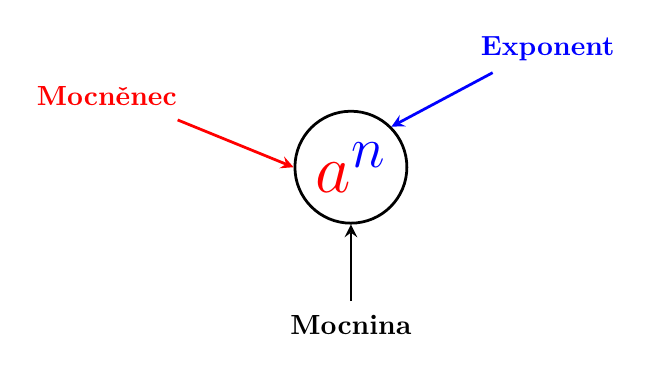
\begin{tikzpicture}[>=stealth, thick]

% uzel s mocninou
\node[circle, draw=black, line width=1pt,
      minimum size=0.5cm, font=\Huge] (exp) {$\textcolor{red}{a}^{\textcolor{blue}{n}}$};


% popisky
\node[red, font=\bfseries] at (-3.1,0.9) {Mocněnec};
\node[blue, font=\bfseries] at (2.5,1.5) {Exponent};
\node[font=\bfseries] at (0,-2) {Mocnina};

% šipky
\draw[->, red, line width=1pt] (-2.2,0.6) -- (exp.west);
\draw[->, blue, line width=1pt] (1.8,1.2) -- (exp.north east);
\draw[->, black, line width=1pt] (0,-1.7) -- (exp.south);

\end{tikzpicture}
\end{center}


\textbf{Z definice vyplývají dvě věci:}
\begin{enumerate}[label=\arabic*)]
    \item \(a^1 = a\), tj. pro všechna reálná čísla \(a\), která jsou umocněna na první, platí, že výsledkem je původní číslo.
    \item \(1^n = 1\) a \(0^n = 0\), tj. pro každé přirozené číslo \(n\) platí, že když umocníme 1, dostáváme stále 1, a při umocňování nuly dostáváme vždy nulu (s výjimkou nedefinovaného výrazu \(0^0\)).
\end{enumerate}


Umocňovat můžeme jak kladná, tak i záporná čísla, a to na sudé i liché exponenty. 
Metodou jednoduchých výpočtů zjistíme tři základní pozorování:

\begin{examplebox}
\[
2^2 = 2 \cdot 2 = 4, \qquad 
2^3 = 2 \cdot 2 \cdot 2 = 8.
\]
Umocněný kladný základ je vždy \textbf{kladný}.
\end{examplebox}

\begin{examplebox}
\[
(-2)^2 = (-2)\cdot(-2) = 4.
\]
Umocnění záporného základu na \textbf{sudý} exponent dává vždy kladný výsledek.
\end{examplebox}

\begin{examplebox}
\[
(-2)^3 = (-2)\cdot(-2)\cdot(-2) = -8.
\]
Umocnění záporného základu na \textbf{lichý} exponent dává vždy záporný výsledek.
\end{examplebox}

\textbf{Shrnutí:}
\[
\begin{aligned}
&a>0,\; n\in\mathbb{N} &\implies &\; a^n>0, \\[6pt]
&a<0,\; n=2k &\implies &\; a^n>0, \\[6pt]
&a<0,\; n=2k+1 &\implies &\; a^n<0.
\end{aligned}
\]

Mocniny nám už značně ulehčují zápis, ale jde to ještě efektivněji a lépe. Abychom mohli počítat i složitější příklady, uvedeme si pravidla pro počítání s mocninami s přirozeným exponent, ty si zároveň i odvodíme.
Pro každé dvě reálná čísla a,b a pro každé přirozená čísla r,s platí:


\textbf{Pravidla pro počítání s mocninami:}
\begin{definitionbox}
\[
\begin{aligned}
a^r \cdot a^s &= a^{r+s}, \\[6pt]
(a^r)^s &= a^{r\cdot s}, \\[6pt]
\frac{a^r}{a^s} &= a^{r-s}, \quad a \neq 0,\; r>s, \\[6pt]
(ab)^r &= a^r \cdot b^r, \\[6pt]
\left(\frac{a}{b}\right)^r &= \frac{a^r}{b^r}, \quad b \neq 0.
\end{aligned}
\]    
\end{definitionbox}


\subsection*{Důkazy pravidel pro mocniny}

% 1. Součin mocnin
\[
a^r \cdot a^s = 
\underbrace{a \cdot a \cdot \ldots \cdot a}_{r}
\cdot
\underbrace{a \cdot a \cdot \ldots \cdot a}_{s}
=
\underbrace{a \cdot a \cdot \ldots \cdot a}_{r+s}
= a^{r+s}
\]

% 2. Mocnina mocniny
\[
(a^r)^s 
=
\left(\overbrace{a \cdot a \cdot \ldots \cdot a}^{r}\right)^s
=
\overbrace{\overbrace{a \cdot a \cdot \ldots \cdot a}^{r}
\cdot
\overbrace{a \cdot a \cdot \ldots \cdot a}^{r}
\cdot
\ldots
\cdot
\overbrace{a \cdot a \cdot \ldots \cdot a}^{r}}^{s}
= \overbrace{a \cdot a \cdot \ldots \cdot a}^{r \cdot s} = a^{r \cdot s}
\]

% 3. Podíl mocnin
\[
\frac{a^r}{a^s} =
\frac{\overbrace{a \cdot a \cdot \ldots \cdot a}^{r}}
     {\underbrace{a \cdot a \cdot \ldots \cdot a}_{s}}
= 
\frac{\overbrace{a \cdot a \cdot \ldots \cdot a}^{s}
      \cdot \overbrace{a \cdot a \cdot \ldots \cdot a}^{r-s}}
     {\underbrace{a \cdot a \cdot \ldots \cdot a}_{s}}
= a^{r-s}, \quad r>s
\]

% 4. Mocnina součinu
\[
(ab)^r = \overbrace{(ab)\cdot (ab)\cdot \ldots \cdot (ab)}^{r\text{-krát}}
\overset{\text{asociativita}}{=}
\left(\overbrace{a \cdot a \cdot \ldots \cdot a}^{r}\right)
\cdot
\left(\overbrace{b \cdot b \cdot \ldots \cdot b}^{r}\right)
= a^r \cdot b^r
\]

% 5. Mocnina podílu
\[
\left(\frac{a}{b}\right)^r =
\overbrace{\left(\frac{a}{b}\right)\cdot \left(\frac{a}{b}\right)\cdot \ldots \cdot \left(\frac{a}{b}\right)}^{r\text{-krát}}
\overset{\text{asociativita}}{=}
\frac{\overbrace{a \cdot a \cdot \ldots \cdot a}^{r}}
     {\underbrace{b \cdot b \cdot \ldots \cdot b}_{r}}
= \frac{a^r}{b^r}
\]


\subsection{Mocniny s celočíselným exponentem}

Doposud jsme umocňovali pouze na přirozené číslo $n \in \mathbb{N}$. 
Nyní definici rozšíříme na všechny celé exponenty $n \in \mathbb{Z}$.

\begin{definitionbox}
Pro všechna reálná čísla $a \neq 0$ a celé číslo $n$ definujeme:
\[
a^0 = 1, \qquad 
a^{-n} = \frac{1}{a^n}, \quad n \in \mathbb{N}.
\]
\end{definitionbox}

Tedy kromě přirozených exponentů připouštíme i nulu a záporná čísla.

\begin{examplebox}
\[
5^0 = 1, \qquad 
2^{-3} = \frac{1}{2^3} = \frac{1}{8}, \qquad 
(-3)^{-2} = \frac{1}{(-3)^2} = \frac{1}{9}.
\]
\end{examplebox}

\textbf{Vysvětlení:}  
- Definice $a^0 = 1$ je přirozená, protože platí pravidlo
\[
\frac{a^m}{a^m} = a^{m-m} = a^0 = 1.
\]
- Definice $a^{-n} = \tfrac{1}{a^n}$ je přirozená, protože zachovává pravidlo
\[
\frac{a^m}{a^n} = a^{m-n}.
\]

\begin{examplebox}
Ověřme:
\[
\frac{2^3}{2^5} = \frac{8}{32} = \frac{1}{4}, 
\qquad 
\text{a současně } \quad 2^{3-5} = 2^{-2} = \frac{1}{2^2} = \frac{1}{4}.
\]
\end{examplebox}

\textbf{Shrnutí:}  
\[
a^n =
\begin{cases}
\underbrace{a \cdot a \cdot \ldots \cdot a}_{n\text{-krát}}, & n > 0, \\[6pt]
1, & n = 0, \\[6pt]
\dfrac{1}{a^{-n}}, & n < 0, \; a \neq 0.
\end{cases}
\]


\subsection{Mocniny desítky a vědecký zápis čísla}

Mocniny desítky $10^n$ jsou v praxi velmi užitečné, protože nám umožňují zapsat velmi velká nebo velmi malá čísla stručně a přehledně.

\begin{definitionbox}
Platí:
\[
10^n = \underbrace{10 \cdot 10 \cdot \ldots \cdot 10}_{n\text{-krát}}, 
\qquad 
10^{-n} = \frac{1}{10^n}.
\]
\end{definitionbox}

\begin{examplebox}
\[
10^3 = 1000, \quad 10^6 = 1\,000\,000, \quad 10^{-2} = 0{,}01.
\]
\end{examplebox}


\textbf{Vědecký (exponenciální) zápis čísla:}

Každé číslo lze zapsat ve tvaru
\[
a \cdot 10^n,
\]
kde $1 \leq a < 10$ a $n \in \mathbb{Z}$.

\begin{examplebox}
\[
5\,000\,000 = 5 \cdot 10^6, \qquad
0{,}00032 = 3{,}2 \cdot 10^{-4}.
\]
\end{examplebox}


\textbf{Kde se s tím setkáte?}
\begin{itemize}
    \item \textbf{Fyzika:} rychlost světla $c \approx 3{,}0 \cdot 10^8 \,\text{m/s}$, hmotnost elektronu $m_e \approx 9{,}11 \cdot 10^{-31} \,\text{kg}$.
    \item \textbf{Chemie:} Avogadrova konstanta $N_A \approx 6{,}022 \cdot 10^{23}$ částic v 1 molu.
    \item \textbf{Astronomie:} vzdálenosti mezi hvězdami, průměr Slunce $1{,}39 \cdot 10^9 \,\text{m}$.
    \item \textbf{Informatika:} gigabajt $= 10^9$ bajtů.
\end{itemize}

\subsubsection*{Mocniny desítky a předpony jednotek}

Mocniny desítky se běžně používají při označování jednotek.  
Každá mocnina má svou předponu, která zjednodušuje zápis velkých i malých čísel.

\begin{center}
\renewcommand{\arraystretch}{1.3}
\begin{tabular}{|c|c|c|}
\hline
\textbf{Mocnina desítky} & \textbf{Předpona} & \textbf{Symbol} \\ \hline
$10^{12}$ & tera & T \\ \hline
$10^{9}$  & giga & G \\ \hline
$10^{6}$  & mega & M \\ \hline
$10^{3}$  & kilo & k \\ \hline
$10^{2}$  & hekto & h \\ \hline
$10^{1}$  & deka & da \\ \hline
$10^{-1}$ & deci & d \\ \hline
$10^{-2}$ & centi & c \\ \hline
$10^{-3}$ & mili & m \\ \hline
$10^{-6}$ & mikro & $\mu$ \\ \hline
$10^{-9}$ & nano & n \\ \hline
$10^{-12}$ & piko & p \\ \hline
\end{tabular}
\end{center}

\begin{examplebox}
\[
1\,\text{km} = 1000\,\text{m} = 10^3 \,\text{m}, \qquad
1\,\mu\text{m} = 0{,}000001\,\text{m} = 10^{-6}\,\text{m}.
\]
\end{examplebox}

\textbf{Poznámka:} S těmito předponami se studenti setkají ve fyzice, chemii, informatice i v běžném životě (kilometry, kilogramy, megabajty, milimetry).


\subsection{Odmocniny}

Odmocnina je \textbf{inverzní operací} k mocnině.  
Pokud víme, že $b^2 = a$, pak číslo $b$ nazýváme \important{druhá odmocnina} z $a$.  
Což následně můžeme zobecnit, pokud $b^n = a$, pak $b$ je \important{$n$-tá odmocnina} z $a$.

\begin{center}
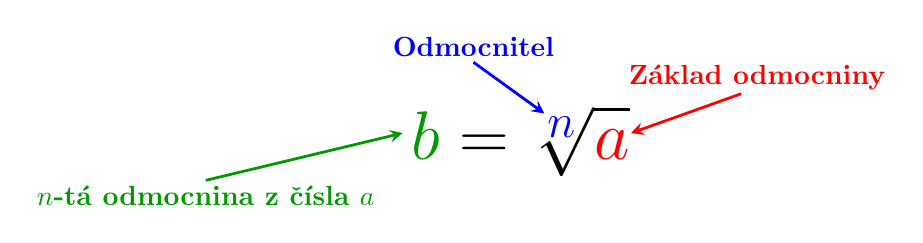
\begin{tikzpicture}[>=stealth, thick]

% hlavní vzorec
\node[font=\Huge] (eq) {${\textcolor{green!60!black}{b}}= \sqrt[\textcolor{blue}n]{\textcolor{red}{a}}$};

% označení b
\node[green!60!black, font=\bfseries] at (-4,-0.7) {$n$-tá odmocnina z čísla $a$};
\draw[->, green!60!black, line width=1pt] (-4,-0.5) -- (-1.5,0.1);

% označení n
\node[blue, font=\bfseries] at (-0.6,1.2) {Odmocnitel};
\draw[->, blue, line width=1pt] (-0.6,1.0) -- (0.3,0.35);

% označení a
\node[red, font=\bfseries] at (3,0.8) {Základ odmocniny};
\draw[->, red, line width=1pt] (2.8,0.6) -- (1.4,0.1);

\end{tikzpicture}
\end{center}


\begin{definitionbox}
Pro $a \geq 0$ a přirozené číslo $n \geq 2$ definujeme:
\[
\sqrt[n]{a} = b \quad \Leftrightarrow \quad b^n = a, \; b \geq 0.
\]
\end{definitionbox}

Zapisujeme pomocí zvláštního znaku $\sqrt{\ }$, kterému říkáme \textbf{odmocnítko}.  
Tento symbol pochází z arabské matematiky a do Evropy se dostal ve středověku.

\begin{examplebox}
\[
\sqrt{25} = 5, \qquad \sqrt[3]{27} = 3, \qquad \sqrt[4]{16} = 2.
\]
\end{examplebox}

\textbf{Pozorování:}  
\begin{itemize}
    \item Sudá odmocnina je definována jen pro nezáporná čísla ($a \geq 0$).  
    \item Lichá odmocnina je definována pro všechna reálná čísla. Např. $\sqrt[3]{-8} = -2$.
\end{itemize}

\textbf{Vlastnosti odmocnin:}
\[
\sqrt[n]{ab} = \sqrt[n]{a} \cdot \sqrt[n]{b}, \qquad
\]
\[
\sqrt[n]{\tfrac{a}{b}} = \frac{\sqrt[n]{a}}{\sqrt[n]{b}}, \quad b \neq 0,
\]
\[
\sqrt[n]{a^m} = a^{\tfrac{m}{n}}.
\]

\begin{examplebox}
\[
\sqrt{36 \cdot 25} = \sqrt{900} = 30, \qquad
\sqrt[3]{\tfrac{8}{27}} = \tfrac{2}{3}.
\]
\end{examplebox}

\textbf{Důležité upozornění:}
\[
\sqrt{a+b} \neq \sqrt{a} + \sqrt{b}.
\]
Například $\sqrt{9+16} = 5$, zatímco $\sqrt{9} + \sqrt{16} = 3+4=7$.

\subsection{Mocniny s racionálním exponent}

Abychom sjednotili zápis mocnin a odmocnin, musíme rozšířit definici i na racionální exponenty.

\begin{definitionbox}
    Pro $a>b$, $m \in \mathbb{Z}$ a $n \in \mathbb{N}$ definujeme:
    \[
    a^{\tfrac{m}{n}} = \sqrt[n]{a^m}.
    \]
\end{definitionbox}

\begin{examplebox}
    \[
    8^{\tfrac{2}{3}} = \sqrt[3]{8^2} = \sqrt[3]{64} = 4, \qquad
    16^{\tfrac{3}{4}} = \sqrt[4]{16^3} = \sqrt[4]{4096} = 8.
    \]
\end{examplebox}

Platí zde stejná pravidla jako pro mocniny s celým exponentem, pouze je dbát 
na definiční obor (např. sudý odmocnitel není definován pro záporné základy).

\subsection{Částečné odmocňování}

Ne vždy vyjde odmocnina přesně jako celé číslo.
Výrazy se nicméně dají často zjednodušit tím, že z pod odmocniny vytkneme tzv \important{Dokonalý čtverec},
nebo obecně n-tou odmocninu.

\begin{examplebox}
    \[
    \sqrt{72} = \sqrt{36 \cdot 2} = \sqrt{36} \cdot \sqrt{2} = 6\sqrt{2}.
    \]
\end{examplebox}

Stejný princip funguje i pro vyšší odmocniny:

\begin{examplebox}
    \[
    \sqrt[3]{54} = \sqrt[3]{27 \cdot 2} = \sqrt[3]{27} \cdot \sqrt[3]{2} = 3\sqrt[3]{2}.
    \]
\end{examplebox}

\textbf{Význam:}
Částečné odmocňování nám umožňuje zapisovat výsledky výpočtů (např. v geometrii a goniometrii) jednodušeji a přehledněji.
Například při výpočtu délky úhlopříčky čtverce se stranou $5$ dostaneme:

\[
u = \sqrt{5^2 + 5^2} = \sqrt{50} = 5\sqrt{2}
\]


\subsection{Usměrňování zlomků}

Občas ve zlomcích můžeme narazit na odmocninu ve jmenoavteli.
Takový zápis není příliš vhodný, proto jej \important{Usměrňujeme} - tedy upravujeme tak, aby ve jmenovateli tato odmocnina nezůstala.

\begin{definitionbox}
\textbf{Usměrnění zlomku} je úprava zlomku tak, že jmenovatel bude racionální číslo (bez odmocniny).
\end{definitionbox}

\begin{examplebox}
    \[
    \frac{1}{\sqrt{2}} = \frac{1}{\sqrt{2}} \cdot \frac{\sqrt{2}}{\sqrt{2}} = \frac{\sqrt{2}}{2}.
    \]
\end{examplebox}

\textbf{Postup}
pro úpravu zlomku s iracionálním jmenovatelem, provádíme tak, že vynásobíme zlomek vhodným zlomkem, který je roven $1$, tak aby se ve jmenovateli odmocnina odstranila.
U jednoduchých odmocnin (např. $\sqrt{2}$) vynásobíme stejnou odmocninou.
U složitějších výrazů využíváme tzv. \textbf{sdružený výraz}.



\textbf{Usměrňování pomocí sdruženého výrazu:}

Pokud máme ve jmenovateli výraz tvaru $\sqrt{a} + \sqrt{b}$, násobíme zlomkem se sdruženým výrazem $\sqrt{a} - \sqrt{b}$.  

\begin{examplebox}
\[
\frac{1}{\sqrt{3}+\sqrt{2}} \cdot \frac{\sqrt{3}-\sqrt{2}}{\sqrt{3}-\sqrt{2}}
= \frac{\sqrt{3}-\sqrt{2}}{(\sqrt{3})^2-(\sqrt{2})^2}
= \frac{\sqrt{3}-\sqrt{2}}{3-2}
= \sqrt{3}-\sqrt{2}.
\]
\end{examplebox}

\textbf{Shrnutí:} \emph{Usměrňování zachovává hodnotu zlomku. Cílem je odstranit odmocniny ze jmenovatele. Používáme buď prosté násobení odmocninou, nebo sdružený výraz.}

\newpage
\subsection{Časté chyby a omyly}

\begin{examplebox}
\[
\sqrt{a+b} \neq \sqrt{a} + \sqrt{b}.
\]  
Např. $\sqrt{9+16} = \sqrt{25} = 5$, ale $\sqrt{9}+\sqrt{16} = 3+4=7$.
\end{examplebox}

\begin{examplebox}
\[
\sqrt{a-b} \neq \sqrt{a} - \sqrt{b}.
\]  
Např. $\sqrt{25-9} = \sqrt{16} = 4$, ale $\sqrt{25}-\sqrt{9} = 5-3=2$.
\end{examplebox}

\begin{examplebox}
Pozor na odmocniny záporných čísel:  
\[
\sqrt{-4} \;\;\; \text{není reálné číslo, ale číslo imaginární (viz. komplexní čísla)}.
\]
\end{examplebox}

Tyto omyly se objevují velmi často a je důležité jim předcházet.

\subsection{Rozšíření na iracionální, reálné a komplexní exponenty}

Doposud jsme se zabývali mocninami s přirozenými, celočíselnými a racionálními exponenty.  
Definici lze však rozšířit dále:

\begin{itemize}
    \item \textbf{Iracionální exponenty:}  
    Pro $a>0$ a $\alpha \in \mathbb{R}$ lze $a^\alpha$ definovat pomocí limit a spojitosti funkcí.  
    Například $\; a^{\sqrt{2}} \;$ je smysluplný zápis, i když $\sqrt{2}$ není racionální.
    
    \item \textbf{Reálné exponenty:}  
    Platí, že $a^x = e^{x \ln a}$, kde $e$ je Eulerovo číslo a $\ln$ přirozený logaritmus.
    
    \item \textbf{Komplexní exponenty:}  
    Definice se rozšiřuje pomocí komplexního logaritmu.  
    Platí vztah
    \[
    e^{ix} = \cos(x) + i \sin(x),
    \]
    který objevil Euler.  
    Tento vztah propojuje exponenciální funkci s goniometrickými funkcemi.
\end{itemize}

\begin{historicalbox}
Jedna z nejslavnějších rovnic matematiky zní:
\[
e^{i\pi} + 1 = 0.
\]
Tento vztah propojuje pět základních matematických konstant: číslo $e$, číslo $\pi$, imaginární jednotku $i$, jedničku a nulu.
\end{historicalbox}




% -----------------------------------------------------------------
% ---------------------- P Ř Í K L A D Y --------------------------
% -----------------------------------------------------------------


\exercisepart
\setcounter{section}{1}

% =========================
% ÚLOHA 1
% =========================
\begin{exercise}[Rychlé mocniny – výpočet z paměti]
    \begin{tasks}(4)
        \task $300^{1}$
        \task $0^{7}$
        \task $2^{5}$
        \task $\left(\tfrac{1}{2}\right)^{5}$
        \task $(-3)^{3}$
        \task $1^{12}$
        \task $(-1)^{35}$
        \task $\left(\tfrac{2}{3}\right)^{4}$
    \end{tasks}
\end{exercise}


% =========================
% ÚLOHA 2
% =========================
\begin{exercise}[Pravdivost tvrzení – znaménko a hodnoty]
    Rozhodni, zda platí (ano/ne).  
    \begin{tasks}(3)
        \task $\left(\tfrac{1}{3}\right)^{30} > 0$
        \task $(-5)^{15} > 0$
        \task $\left(-\tfrac{1}{5}\right)^{22} > 0$
        \task $0^{13} > 0$
        \task $(-3+9)^{11} < 0$
        \task $(-3)^{7}\cdot(-3)^{8} < 0$
    \end{tasks}
\end{exercise}


% =========================
% ÚLOHA 3
% =========================
\begin{exercise}[Mocniny s nulovým exponentem]
    Vypočítej z paměti:
    \begin{tasks}(6)
        \task $2x^{0}$
        \task $(2x)^{0}$
        \task $2^{0} \cdot x$
        \task $2 : x^{0}$
        \task $2^{0} : x$
        \task $0^{0}$
    \end{tasks}
\end{exercise}


% =========================
% ÚLOHA 4
% =========================
\begin{exercise}[Mocniny čísla $-1$]
    Vypočítej z paměti:
    \begin{tasks}(6)
        \task $(-1)^{-1}$
        \task $-1^{2}$
        \task $(-1)^{3}$
        \task $(-1)^{-2}$
        \task $(-1)^{2k}$
        \task $(-1)^{2k+1}$
    \end{tasks}
\end{exercise}


% =========================
% ÚLOHA 5
% =========================
\begin{exercise}[Výpočty bez kalkulačky]
    Vypočítej (bez použití kalkulačky):
    \begin{tasks}(2)
        \task $\left(\tfrac{1}{2}\right)^{-2} + 2^{-1} + (-1)^{5} \cdot \left(-\tfrac{1}{2}\right)^{-2}$
        \task $(0.1)^{-1} - 2^{-2} + \left(-\tfrac{1}{2}\right)^{-4} - \tfrac{1^{-4}}{2} - (-1)^{-1}$
        \task $0.2^{-1} - (-1^{-2}) - \tfrac{1}{2^{-1}} + \tfrac{1^{-5}}{2} - \left(-\tfrac{1}{2}\right)^{-1}$
        \task $\left\{\left[\tfrac{1^{-2}}{2}\right]^{-1} - (3^{-1})^{-2} + 1\right\}$
        \task $\left[2 - \left(\tfrac{1}{3}\right)^{-2}\right]^{2}$
        \task $\left(2^{-2} + 4^{-1}\right)^{2}$
        \task $(0.02)^{-3} \cdot \left[(0.1)^{-2}\right]^{-1}$
        \task $\left(\tfrac{2}{3}\right)^{-2} - \left(-\tfrac{1}{4}\right)^{2} - (0.4)^{-1}$
     \end{tasks}
\end{exercise}


% =========================
% ÚLOHA 6
% =========================
\begin{exercise}[Výpočty s mocninami]
    Vypočítej:
    \begin{tasks}(3)
        \task $\dfrac{2^{5}\cdot 2^{7}}{2^{10}}$
        \task $\dfrac{(-3)^{3}\cdot (-3)^{6}}{(-3)^{5}\cdot 3^{2}}$
        \task $\dfrac{(2^{3}\cdot 3^{2})^{3}}{(2\cdot 3)^{5}}$
        \task $\dfrac{(4^{3}\cdot 2^{-2})}{(8 \cdot 2^{2})}$
        \task $\left(\tfrac{-3^{2}}{(-3)^{3}}\right)^{4}$
        \task $\dfrac{(5^{-1}\cdot 25^{2})}{(125^{-1})}$  
        \task $\left(\tfrac{2^{2}}{5}\right)^{5} \cdot \left(\tfrac{-5^{2}}{2^{3}}\right)^{3}$
        \task $\dfrac{|{-2}|^{5} \cdot |{(-5)}^{5}|}{[(-2)\cdot (-5)]^{3}}$
        \task $\dfrac{(2^{2} - |{-5}|)^{20}}{(-2)^{3}\cdot (-5)^{2}}$
    \end{tasks}
\end{exercise}


% =========================
% ÚLOHA 7
% =========================
\begin{exercise}[Vyjádři jako mocniny se základem $2$ nebo $3$ a vypočítej]
% Tip pro žáky (nezobrazí se): 
% 81=3^4,\; 64=2^6,\; 96=2^5\cdot3,\; 36=2^2\cdot3^2,\; 6^3=2^3\cdot3^3,\;
% 128=2^7,\; 8=2^3,\; 9=3^2,\; 16=2^4,\; 72=2^3\cdot3^2,\; 27=3^3
    \begin{tasks}(2)
        \task $\left(\dfrac{(2^{10}\!\cdot 3)^{2}}{2\cdot 3^{13}}\right)\cdot\left(\dfrac{81}{64}\right)^{3}$
        \task $\left(\dfrac{9^{5}\cdot 2^{7}}{27^{2}\cdot 96}\right)\cdot\left(\dfrac{36}{6^{3}}\right)$
        \task $\left(\dfrac{128\cdot 3^{5}}{81\cdot 8}\right)^{3} : \left(\dfrac{(16\cdot 3^{5})^{2}}{9^{4}}\right)$
        \task $\left(\dfrac{8^{4}\cdot 9^{5}}{72^{3}}\right) : \left(\dfrac{2\cdot 3^{6}}{27}\right)$
    \end{tasks}
\end{exercise}


\setcounter{section}{2}
% =========================
% ÚLOHA 8
% =========================
\begin{exercise}[Zjednodušte zapsáním v podobě mocnin prvočísel]
    \begin{tasks}(1)
        \task $\dfrac{2^{9}\cdot 10^{5}\cdot 15^{4}\cdot 18^{3}}{3^{7}\cdot 5^{5}\cdot 20^{4}\cdot 24^{3}}$
        \task $\dfrac{3^{8}\cdot 12^{4}\cdot 25^{3}\cdot 8^{2}}{2^{10}\cdot 9^{5}\cdot 5^{4}\cdot 30^{2}}$
        \task $\dfrac{2^{6}\cdot 5^{3}\cdot 27^{2}\cdot 50^{4}}{3^{7}\cdot 10^{5}\cdot 75^{3}\cdot 4^{2}}$
        \task $\dfrac{6^{5}\cdot 14^{3}\cdot 45^{2}\cdot 8^{4}}{2^{9}\cdot 3^{6}\cdot 7^{2}\cdot 60^{3}}$
    \end{tasks}
\end{exercise}


\setcounter{section}{3}
% =========================
% ÚLOHA 9
% =========================
\begin{exercise}[Uprav výrazy]
    \begin{tasks}(2)
        \task $(3a^7b^{-2}c^{-3})\cdot(4a^{-6}b^2c^{-1})$
        \task $\left(\frac{1}{2}a^{-2}b^3c\right)^{-3} : (4a^4b^{-8}c^{-3})$
        \task $\left(\dfrac{ab^{-3}}{c^4}\right)^{-2}$ 
        \task $\dfrac{9a^6b^{-5}}{c^{-3}} : \left(\dfrac{3^{-1}b^3}{a^2c^{-4}}\right)^{-2} $   
        \task $\dfrac{2(ab)^{3}}{3a^{2}b}\cdot\dfrac{(3a^{3}b^{2})^{2}}{a^{5}b^{3}}$
        \task $\dfrac{5a^{3}b^{7}}{2ab^{6}}\cdot\left(\dfrac{2a^{2}b^{3}}{ab^{2}}\right)^{3}$
        \task $\dfrac{2x^{5}y^{3}}{(2x^{2}y)^{2}} : \left(\dfrac{xy}{2xy^{2}}\right)^{3}$
        \task $\dfrac{7x^{4}y^{7}}{8x^{3}y} : \dfrac{(x^{2}y)^{4}}{(2x^{3}y^{2})^{3}}$    
    \end{tasks}
\end{exercise}


% =========================
% ÚLOHA 10
% =========================
\begin{exercise}[Zjednoduš a určete, kdy mají výrazy smysl]
    U každého výrazu proveďte úpravu a \textbf{určete podmínky smyslu} (zakázané hodnoty proměnných — např. proměnné v
    jmenovateli a se záporným exponentem nesmí být $0$).
    \begin{tasks}(2)
        \task $(x^{2})^{-1} : 9\,(x^{-3})^{2}$
        \task $\dfrac{(x^{4}y^{-3})^{-2}}{(x^{3})^{-3}\cdot y^{5}}$
        \task $(0.8)^{-1}\cdot a^{2}b^{-3}\cdot 1.5\,a^{-2}b^{5}$
        \task $\left(\dfrac{a^{2}b^{-3}}{c^{-2}d^{3}}\right)^{-1}\cdot \left(\dfrac{c^{4}d^{-1}}{a^{-3}b^{2}}\right)^{2}$
        \task $\dfrac{\left[n^{-2}\cdot 3n^{3}\cdot (6n)^{-1}\right]^{-2}}{(2n^{-1})^{0}}$
        \task $\left[m^{4}\cdot \left(\tfrac{2}{m}\right)^{5}\cdot \left(\tfrac{m^{2}}{4}\right)^{-3}\cdot \tfrac{1}{16}\right]^{-1}$
        \task $\dfrac{(p^{-2}q^{3})^{-2}\cdot (pq^{-1})^{4}}{(p^{3}q)^{-1}}$
        \task $\left[\dfrac{(2x^{-3}y^{2})^{-1}}{(4x^{-1}y^{-2})^{2}}\right]^{-1} \cdot (xy^{-1})^{0}$
    \end{tasks}
\end{exercise}

\newpage
% =========================
% ÚLOHA 11
% =========================
\begin{exercise}[Zjednodušte následující výrazy]
    \begin{tasks}(2)
        \task $\dfrac{x^{5}\cdot\bigl(x^{n}\cdot 6 \cdot y^{4n}\bigr)^{3}}{9 \cdot y^{4n}\cdot\bigl(x^{5}\cdot 2 \cdot y^{6}\bigr)^{2}}$    
        \task $\dfrac{(16b^{3}a^{-1})^{-3}}{(a^{3}b^{-2}\cdot 4)^{-2}}$
        \task $\dfrac{\bigl(27r^{3}s^{4}\bigr)^{\,n-1}}{\bigl(3rs^{-2}\bigr)^{\,3x+1}}$
        \task $\dfrac{(50p^{-2}q^{3})^{\,2n+1}\cdot(5pq^{-4})^{\,n}}{(10p^{-1}q^{2})^{\,3n-2}}$
    \end{tasks}
\end{exercise}


\setcounter{section}{4}
% =========================
% ÚLOHA 12
% =========================
\begin{exercise}[Vědecký zápis a převody jednotek]
    Uvedené údaje vyjádřete v jednotkách uvedených v závorce a zapište ve tvaru $a \cdot 10^n$, kde $1 \leq a < 10$, $n \in \mathbb{Z}$.
    \begin{tasks}(2)
        \task $6 378\;km$, (m)
        \task $250\;hl$, (l)
        \task $650\;MW$, (W)
        \task $27 \; m^3$, (l)
    \end{tasks}
\end{exercise}


\setcounter{section}{5}
% =========================
% ÚLOHA 13
% =========================
\begin{exercise}[Výpočty se zápornými exponenty – zlomky]
    Vypočítej zpaměti:
    \begin{tasks}(3)
        \task $\left(\tfrac{1}{5}\right)^{-2}$
        \task $\left(-\tfrac{1}{3}\right)^{-2}$
        \task $\left(-\tfrac{1}{3}\right)^{-3}$
        \task $\left(\tfrac{6}{5}\right)^{-2}$
        \task $\left(-\tfrac{2}{3}\right)^{-3}$
        \task $\left(\tfrac{4}{7}\right)^{-3}$
    \end{tasks}
\end{exercise}


% =========================
% ÚLOHA 14
% =========================
\begin{exercise}[Vypočítejte následující výrazy]
    \begin{tasks}(3)
        \task $2^{\tfrac{3}{2}} \cdot 2^{\tfrac{4}{3}} \cdot 2^{\tfrac{7}{6}}$
        \task $\left(\dfrac{4}{9}\right)^{-\tfrac{3}{2}} \cdot \left(\dfrac{27}{8}\right)^{\tfrac{2}{3}}$
        \task $\left(\dfrac{5^{2}\cdot 2^{-3}}{10^{-1}}\right)^{\tfrac{3}{2}}$
        \task $\dfrac{(2^{3}\cdot 3^{2})^{\tfrac{1}{2}}}{6^{\tfrac{3}{2}}}$
        \task $\dfrac{(5^{\frac{3}{5}})^{\tfrac{3}{2}}}{5^{\frac{4}{10}}}$
        \task $\dfrac{(3^{\frac{30}{7}} \cdot 4^{\frac{18}{7}})^{\frac{7}{6}}}{36^{\frac{5}{2}}}$
    \end{tasks}
\end{exercise}


% =========================
% ÚLOHA 15
% =========================
\begin{exercise}[Výpočty se zápornými exponenty – celé číslo a desetinná čísla]
    Vypočítej zpaměti:
    \begin{tasks}(3)
        \task $(-2)^{-5}$
        \task $-2^{-5}$
        \task $(0.75)^{-1}$
        \task $\left(-\tfrac{3}{4}\right)^{-2}$
        \task $(-0.5)^{-3}$
        \task $-0.5^{-3}$
    \end{tasks}
\end{exercise}


\setcounter{section}{6}
% =========================
% ÚLOHA 16
% =========================
\begin{exercise}[Výpočty se zápornými exponenty – odmocniny]
    Vypočítej zpaměti:
    \begin{tasks}(3)
        \task $(\sqrt{3})^{-2}$
        \task $\left(\tfrac{1}{\sqrt{2}}\right)^{-3}$
        \task $\left(-\tfrac{1}{\sqrt{2}}\right)^{-2}$
        \task $\left(-\tfrac{1}{\sqrt{3}}\right)^{-3}$
        \task $(\sqrt{5})^{0}$
        \task $\left(\tfrac{\sqrt{2}}{\sqrt{3}}\right)^{-4}$
    \end{tasks}
\end{exercise}

\newpage
% =========================
% ÚLOHA 17
% =========================
\begin{exercise}[Vyjádřete v nejjednodušším tvaru]
    \begin{tasks}(2)
        \task $\left(\sqrt{5} - 2\right)^{-1}$
        \task $\left(2 - \sqrt{6}\right)^{-2}$
        \task $\left(\sqrt{3} - \sqrt{2}\right)^{-2}$
        \task $40\left(5 - \sqrt{5}\right)^{-2}$
        \task $\left(\dfrac{1}{\sqrt{2}} - \dfrac{1}{\sqrt{3}}\right)^{-1}$  % středně těžký
        \task $\left(\dfrac{1}{\sqrt{2}+\sqrt{3}} + \dfrac{1}{\sqrt{2}-\sqrt{3}}\right)^{-2}$ % těžký
    \end{tasks}
\end{exercise}



% =========================
% ÚLOHA 18
% =========================
\begin{exercise}[Vypočítejte]
    \begin{tasks}(2)
        \task $\sqrt[4]{2}\cdot \sqrt[4]{8}$
        \task $\sqrt[3]{16}:\sqrt[3]{2}$        
        \task $(3\sqrt[3]{16}+2\sqrt[3]{54})\cdot \sqrt[3]{4}$
        \task $\bigl(\sqrt[4]{3}+\sqrt[4]{2}\bigr)\cdot \bigl(\sqrt[4]{27}-\sqrt[4]{8}\bigr)$
        \task $\sqrt[5]{32}\cdot \sqrt[5]{4}$
        \task $\dfrac{\sqrt[6]{64}}{\sqrt[6]{2}}$
        \task $(2\sqrt[3]{81}-\sqrt[3]{24})\cdot \sqrt[3]{3}$
        \task $\bigl(\sqrt[4]{18}+\sqrt[4]{8}\bigr)^{2}$
    \end{tasks}
\end{exercise}


% =========================
% ÚLOHA 19
% =========================
\begin{exercise}[Upravte výrazy]
    \begin{tasks}(2)
        \task $\sqrt{12+4}$
        \task $\sqrt{-8+33}$
        \task $\sqrt{26^{2}}+27$      % záměrně mimo odmocnitko jako na obrázku
        \task $\sqrt{169}-\sqrt{225}$
        \task $\sqrt{361}+\sqrt{1}$
        \task $\sqrt{(4+9)^{2}}$
        \task $\sqrt{20\cdot 20}$
        \task $\dfrac{50-\sqrt{225}}{\sqrt{49}}$
        \task $\dfrac{\sqrt{64}\cdot\sqrt{36}}{\sqrt{9}\cdot\sqrt{256}}$
        \task $\left(\dfrac{1}{\sqrt{2}+\sqrt{3}}+\dfrac{1}{\sqrt{2}-\sqrt{3}}\right)^{-1}$
        \task $\sqrt{50+20\sqrt{6}}-\sqrt{8}$
        \task $\dfrac{\sqrt{45}-\sqrt{20}}{\sqrt{5}-\sqrt{4}}$
        \task $2\cdot(3^2 - 2^3)^{99} - 1\cdot \sqrt{5^2 - 3^2}$
        \task $\left(\sqrt{\frac{64}{81}} - \frac{2}{3}\right)^2 : \frac{2}{9}$
    \end{tasks}
\end{exercise}


\setcounter{section}{7}
% =========================
% ÚLOHA 20
% =========================
\begin{exercise}[Částečné odmocňování]
    Zjednodušte výrazy:
    \begin{tasks}(3)
        \task $\sqrt{288}$
        \task $\sqrt{5000}$
        \task $\sqrt{882}$
        \task $\sqrt{2\cdot 75}$
        \task $\sqrt{\tfrac{98}{8}}$
        \task $\dfrac{\sqrt{147}\cdot\sqrt{63}}{\sqrt{21}}$
        \task $\sqrt[3]{2160}$
        \task $\sqrt[3]{8748}$
        \task $\sqrt[4]{648}$
        \task $\dfrac{\sqrt[3]{128}\cdot \sqrt[3]{250}}{\sqrt[3]{2}}$
        \task $\sqrt{\dfrac{800}{18}}$
        \task $\sqrt[3]{\dfrac{1458}{24}}$
    \end{tasks}
\end{exercise}


\newpage
\setcounter{section}{8}
% =========================
% ÚLOHA 21
% =========================
\begin{exercise}[Usměrňování zlomků]
    Usměrněte následující výrazy:
    \begin{tasks}(3)
        \task $\dfrac{1}{\sqrt{3}}$
        \task $\dfrac{2}{\sqrt{5}}$
        \task $\dfrac{1}{2\sqrt{7}}$
        \task $\dfrac{5}{\sqrt{12}}$
        \task $\dfrac{\sqrt{2}}{\sqrt{5}}$
        \task $\dfrac{1}{\sqrt{3}+\sqrt{2}}$
        \task $\dfrac{2}{\sqrt{6}-\sqrt{2}}$
        \task $\dfrac{\sqrt{5}}{\sqrt{2}+\sqrt{3}}$
        \task $\dfrac{15}{2\sqrt{3}-3}$
        \task $\frac{\sqrt{6}-2\sqrt{2}}{\sqrt{15}-2\sqrt{5}}$
        \task $\dfrac{3}{\sqrt[3]{2}}$
        \task $\dfrac{1}{\sqrt[3]{5}+\sqrt[3]{2}}$
    \end{tasks}
\end{exercise}


% =========================
% ÚLOHA 22
% =========================
\begin{exercise}[Usměrňování zlomků – náročnější příklady]
    Usměrněte následující výrazy:
    \begin{tasks}(2)
        \task $\dfrac{1}{\sqrt{7}+\sqrt{2}+\sqrt{5}}$
        \task $\dfrac{2}{\sqrt{3}-\sqrt{2}+\sqrt{5}}$
        \task $\dfrac{1}{\sqrt{2}+\sqrt{3}+\sqrt{6}}$
        \task $\dfrac{1}{\sqrt{a}+\sqrt{b}+\sqrt{c}}$
        \task $\dfrac{\sqrt[3]{2}}{\sqrt[3]{4}+\sqrt[3]{2}}$
        \task $\dfrac{1}{\sqrt[3]{5}+\sqrt[3]{2}}$
        \task $\dfrac{1}{\sqrt[3]{a}+\sqrt[3]{b}+\sqrt[3]{c}}$
        \task $\dfrac{1}{\sqrt{2}+\sqrt{3}}+\dfrac{1}{\sqrt{3}+\sqrt{5}}+\dfrac{1}{\sqrt{5}+\sqrt{2}}$
    \end{tasks}
\end{exercise}


\setcounter{section}{9}
% =========================
% ÚLOHA 23 – Závěrečný MIX
% =========================
\begin{exercise}[Spočítejte a vhodně zjednodušte]
    \begin{tasks}(2)
        \task $\dfrac{1}{6}\cdot\sqrt{0.01}\;+\;\dfrac{3}{5}\;:\;\!\left(-1\tfrac{5}{7}\right)$
        \task $\dfrac{\left(-1\tfrac{1}{3}\right)^{2}\;-\;\dfrac{5}{6}\cdot 0.3}{\dfrac{5}{9}\;-\;\sqrt{2\tfrac{7}{9}}}$
        \task $\dfrac{\dfrac{2}{\sqrt{49}}\;+\;\dfrac{8}{9}\cdot 0.5^{2}}{3\tfrac{1}{3}\;:\;1\tfrac{2}{5}\;-\;2}$
        \task $\dfrac{\dfrac{1}{\sqrt{25}}\;-\;\big(\sqrt{0.09}-\sqrt{\tfrac{1}{16}}\big)}{\left(-\tfrac{4}{5}\right)\;:\;\left(\tfrac{7}{9}-\tfrac{11}{18}\right)}$
        \task $\dfrac{\sqrt{0.04}\;:\;\left(\tfrac{2}{3}-\tfrac{1}{5}\right)\;-\;\tfrac{3}{7}}{\tfrac{8}{11}\;-\;\left(-\tfrac{1}{2}\right)^{2}\;+\;\tfrac{13}{22}}$
        \task $\dfrac{\left[\tfrac{1}{9}-\left(\tfrac{5}{6}\right)^{2}\right]\;:\;\left(-\tfrac{2}{3}\right)}{\tfrac{2}{3}\cdot 0.25\;-\;\sqrt{\tfrac{9}{16}}}$
        \task $\dfrac{\left(\tfrac{1}{4}\right)^{2}\cdot 2\tfrac{2}{3}\;-\;1\tfrac{1}{2}\cdot \dfrac{\sqrt{9}}{5}}{\dfrac{2}{3}\;-\;0.5^{2}\cdot\left(-\tfrac{2}{5}\right)}$
        \task $\dfrac{\left[\dfrac{2}{\sqrt{25}}+\left(-\tfrac{1}{6}\right)\right]\;:\;0.1}{1\;-\;\dfrac{(-4)^{2}}{9}\cdot 0.6}$
        % --- několik „chuťovek“ navíc ---
        \task $\dfrac{\left(\tfrac{3}{2}\right)^{-2}+\left(\tfrac{2}{3}\right)^{2}-\left(-\tfrac{1}{2}\right)^{-1}}{\sqrt{\tfrac{1}{4}}-\sqrt{0.01}}$
        \task $\left(\dfrac{\sqrt{48}}{\sqrt{3}}-\dfrac{\sqrt{75}}{5}\right):\left(\dfrac{1}{\sqrt{3}+\sqrt{2}}+\dfrac{1}{\sqrt{3}-\sqrt{2}}\right)$
        \task $\dfrac{\left(0.2^{-1}-\sqrt{\tfrac{1}{25}}\right)\cdot\left(\sqrt{8}-\sqrt{2}\right)}{\left(\tfrac{9}{4}\right)^{-\tfrac{1}{2}}+\left(\tfrac{16}{25}\right)^{\tfrac{1}{2}}}$
        \task $\dfrac{\left(\sqrt{5}-\sqrt{2}\right)^{2}-\left(\sqrt{3}-1\right)\left(\sqrt{3}+1\right)}{\dfrac{1}{\sqrt{8}}+\dfrac{1}{\sqrt{18}}}$
    \end{tasks}
\end{exercise}


\begin{exercise}[Zjednodušte]
    \begin{tasks}(2)
        \task $\left(\dfrac{1}{b-\sqrt{a}} + \dfrac{1}{b+\sqrt{a}}\right) : \dfrac{\sqrt{\frac{1}{9^{-1}}}a^{-2}b^{-1}}{a^{-2}-a^{-1}b^{-2}}$
        \task $\left(\sqrt{\sqrt[3]{\dfrac{x-y}{x+y}}}\right)^2 : \sqrt{\dfrac{x+y}{x-y}\sqrt[3]{\dfrac{x+y}{x-y}}}$
        \task $\sqrt{\dfrac{a \cdot \sqrt[3]{b}}{\sqrt[3]{a \cdot \sqrt{b}}}}$
        \task $\sqrt[5]{\sqrt{m} \cdot \sqrt[3]{\frac{1}{m}} \cdot \sqrt[5]{m^{-2}}}$
    \end{tasks}
\end{exercise}


\newpage
\setcounter{section}{10}
% =========================
% BONUS
% =========================
\begin{exercise}[BONUS: Řetězová odmocnina]
    Vypočítej:
    \[
    S=\sqrt{\dfrac{3}{\sqrt{\dfrac{45}{\sqrt{\dfrac{250}{\sqrt{\dfrac{400}{\sqrt{16}}}}}}}}}
    \]
\end{exercise}


% =========================
% BONUS
% =========================
\begin{exercise}[BONUS: zobecnění]
Najděte všechna $n \in \mathbb{N}$, pro která je $2^{n}+1$ dělitelné $3$.
% Nápověda (pro učitele): Rozlišit liché/sudé n podle kongruence 2^n \equiv (-1)^n \pmod 3.
\end{exercise}


% =========================
% BONUS
% =========================
\begin{exercise}[BONUS: poslední cifra]
Určete poslední cifru čísla $7^{2025}$.
\end{exercise}


% =========================
% BONUS
% =========================
\begin{exercise}[BONUS: n-tá mocnina z \(n^{\,n-2}\)]
Najděte všechna celá čísla \(n>2\), pro která je číslo \(n^{\,n-2}\) \(n\)-tou mocninou celého čísla.
\end{exercise}


% =========================
% BONUS
% =========================
\begin{exercise}[BONUS: mocniny na tabuli]
Na tabuli jsou napsána čísla $1, \sqrt{2}, \sqrt{3}$.  
V každém kroku smažeme čísla $a, b, c$ napsaná na tabuli a nahradíme je součiny $ab, \; bc, \; ca$.  

Zjistěte, zda se po několika krocích může stát, že se na tabuli znovu objeví některé přirozené číslo.
\end{exercise}

\end{document}